% Options for packages loaded elsewhere
\PassOptionsToPackage{unicode}{hyperref}
\PassOptionsToPackage{hyphens}{url}
\PassOptionsToPackage{dvipsnames,svgnames,x11names}{xcolor}
%
\documentclass[
  11pt,
]{article}
\usepackage{amsmath,amssymb}
\usepackage{iftex}
\ifPDFTeX
  \usepackage[T1]{fontenc}
  \usepackage[utf8]{inputenc}
  \usepackage{textcomp} % provide euro and other symbols
\else % if luatex or xetex
  \usepackage{unicode-math} % this also loads fontspec
  \defaultfontfeatures{Scale=MatchLowercase}
  \defaultfontfeatures[\rmfamily]{Ligatures=TeX,Scale=1}
\fi
\usepackage{lmodern}
\ifPDFTeX\else
  % xetex/luatex font selection
\fi
% Use upquote if available, for straight quotes in verbatim environments
\IfFileExists{upquote.sty}{\usepackage{upquote}}{}
\IfFileExists{microtype.sty}{% use microtype if available
  \usepackage[]{microtype}
  \UseMicrotypeSet[protrusion]{basicmath} % disable protrusion for tt fonts
}{}
\makeatletter
\@ifundefined{KOMAClassName}{% if non-KOMA class
  \IfFileExists{parskip.sty}{%
    \usepackage{parskip}
  }{% else
    \setlength{\parindent}{0pt}
    \setlength{\parskip}{6pt plus 2pt minus 1pt}}
}{% if KOMA class
  \KOMAoptions{parskip=half}}
\makeatother
\usepackage{xcolor}
\usepackage[margin=1in]{geometry}
\usepackage{longtable,booktabs,array}
\usepackage{calc} % for calculating minipage widths
% Correct order of tables after \paragraph or \subparagraph
\usepackage{etoolbox}
\makeatletter
\patchcmd\longtable{\par}{\if@noskipsec\mbox{}\fi\par}{}{}
\makeatother
% Allow footnotes in longtable head/foot
\IfFileExists{footnotehyper.sty}{\usepackage{footnotehyper}}{\usepackage{footnote}}
\makesavenoteenv{longtable}
\usepackage{graphicx}
\makeatletter
\def\maxwidth{\ifdim\Gin@nat@width>\linewidth\linewidth\else\Gin@nat@width\fi}
\def\maxheight{\ifdim\Gin@nat@height>\textheight\textheight\else\Gin@nat@height\fi}
\makeatother
% Scale images if necessary, so that they will not overflow the page
% margins by default, and it is still possible to overwrite the defaults
% using explicit options in \includegraphics[width, height, ...]{}
\setkeys{Gin}{width=\maxwidth,height=\maxheight,keepaspectratio}
% Set default figure placement to htbp
\makeatletter
\def\fps@figure{htbp}
\makeatother
\setlength{\emergencystretch}{3em} % prevent overfull lines
\providecommand{\tightlist}{%
  \setlength{\itemsep}{0pt}\setlength{\parskip}{0pt}}
\setcounter{secnumdepth}{-\maxdimen} % remove section numbering
\ifLuaTeX
  \usepackage{selnolig}  % disable illegal ligatures
\fi
\IfFileExists{bookmark.sty}{\usepackage{bookmark}}{\usepackage{hyperref}}
\IfFileExists{xurl.sty}{\usepackage{xurl}}{} % add URL line breaks if available
\urlstyle{same}
\hypersetup{
  pdfauthor={Stefano Alimonti --- stefalimonti@gmail.com},
  colorlinks=true,
  linkcolor={blue},
  filecolor={Maroon},
  citecolor={Blue},
  urlcolor={blue},
  pdfcreator={LaTeX via pandoc}}

\author{Stefano Alimonti --- stefalimonti@gmail.com}
\date{March 2026}

\begin{document}

{
\hypersetup{linkcolor=black}
\setcounter{tocdepth}{2}
\tableofcontents
}
\section{Reader's Guide: Spectral Theory of Carries in Positional
Multiplication}\label{readers-guide-spectral-theory-of-carries-in-positional-multiplication}

\textbf{Stefano Alimonti} --- March 2026

\emph{This is a self-contained overview of the main paper. It walks through the
key ideas using a single worked example and requires no prior familiarity with
the carry-chain literature.}

\begin{center}\rule{0.5\linewidth}{0.5pt}\end{center}

\newpage

\subsection{1. What This Paper Is About}\label{what-this-paper-is-about}

When you multiply two numbers by hand in base \(b\), you write out partial
products and add them column by column, carrying the overflow to the next
column. The carry at each position depends only on the column sum and the carry
from the previous position --- not on anything earlier. This means the sequence
of carries forms a \textbf{Markov chain}.

Diaconis and Fulman (2009) proved that carries in base-\(b\) \emph{addition}
form a Markov chain with a beautiful spectrum: the eigenvalues are exactly
\(1, 1/b, 1/b^2, \ldots, 1/b^n\) when adding \(n+1\) numbers. These are the same
eigenvalues that govern the convergence of the Gilbert-Shannon-Reeds riffle
shuffle --- a deep connection between combinatorics and probability.

\textbf{The question we answer:} What happens when addition is replaced by
multiplication? The column sums in multiplication are \emph{convolutions}
\(\sum_{i+j=k} g_i h_j\) rather than simple sums, and they have a more complex
probabilistic structure. What are the eigenvalues of the carry transfer
operator, and how fast does the chain mix?

\subsubsection{\texorpdfstring{A complete example: \(13 \times 11\) in base
2}{A complete example: 13 \textbackslash times 11 in base 2}}\label{a-complete-example-13-times-11-in-base-2}

Take \(13 = (1101)_2\) and \(11 = (1011)_2\). The grade-school algorithm:

\begin{verbatim}
          1 1 0 1          (13)
        × 1 0 1 1          (11)
        ---------
          1 1 0 1          partial product: 13 × 1
        1 1 0 1 ·          partial product: 13 × 1, shifted left 1
      0 0 0 0 · ·          partial product: 13 × 0, shifted left 2
    1 1 0 1 · · ·          partial product: 13 × 1, shifted left 3
    -----------------
    1 0 0 0 1 1 1 1        = 143
\end{verbatim}

Each column sum is the convolution \(\text{conv}_k = \sum_{i+j=k} g_i h_j\). The
carry propagation:

\begin{longtable}[]{@{}llllll@{}}
\toprule\noalign{}
Pos \(k\) & Column sum & Carry in & Total & Output digit & Carry out \\
\midrule\noalign{}
\endhead
\bottomrule\noalign{}
\endlastfoot
0 & 1 & 0 & 1 & 1 & 0 \\
1 & 1 & 0 & 1 & 1 & 0 \\
2 & 1 & 0 & 1 & 1 & 0 \\
3 & \textbf{3} & 0 & \textbf{3} & 1 & \textbf{1} \\
4 & 1 & \textbf{1} & 2 & 0 & \textbf{1} \\
5 & 1 & \textbf{1} & 2 & 0 & \textbf{1} \\
6 & 1 & \textbf{1} & 2 & 0 & \textbf{1} \\
\end{longtable}

The carry sequence is \(0, 0, 0, 0, 1, 1, 1, 1\). At position 3, the column sum
(= 3) exceeds the base (= 2), and a carry is born. It then persists. \emph{How
quickly does a typical carry chain settle into a steady state? What controls the
rate?} These are the questions we answer.

\begin{figure}
\centering
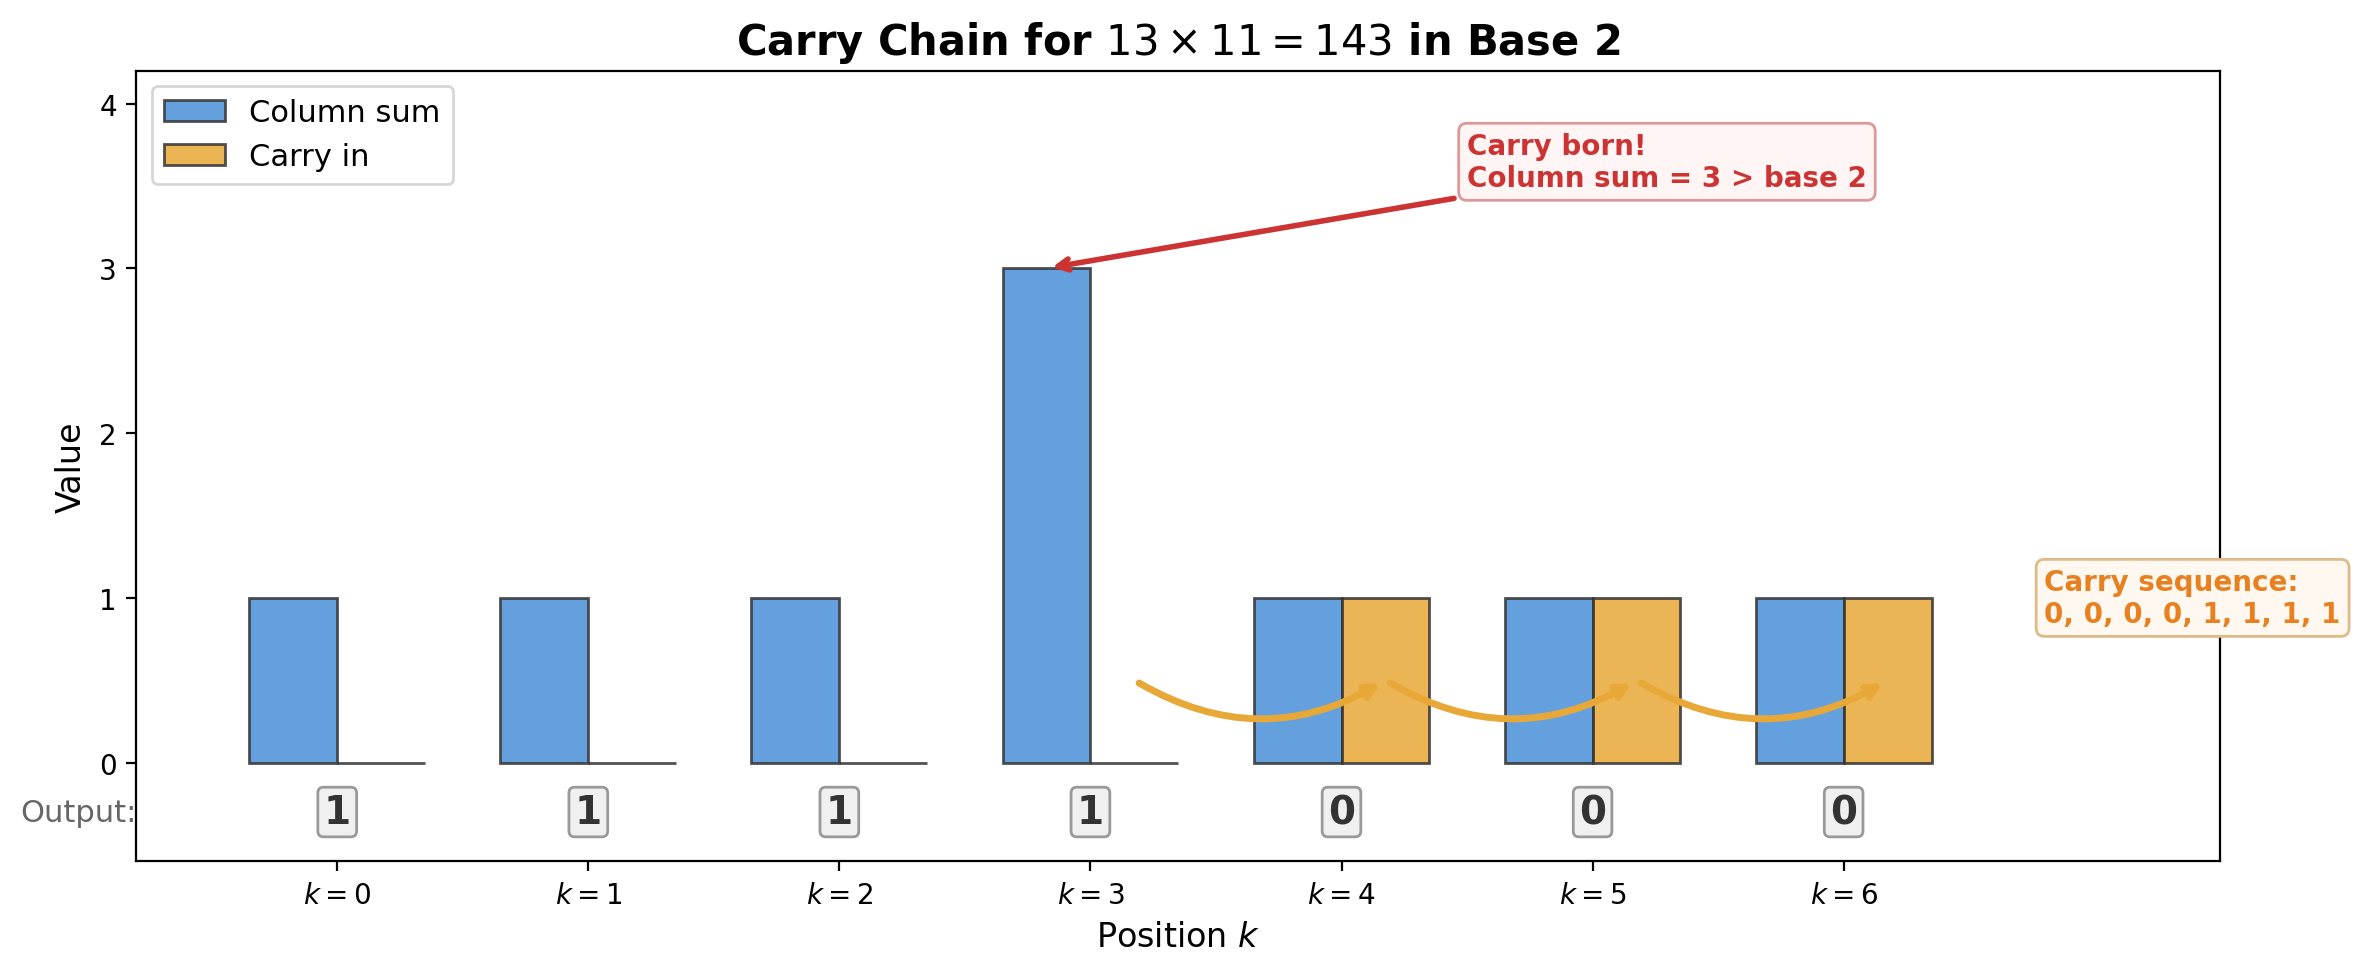
\includegraphics{../figures/fig_carry_chain.png}
\caption{Carry chain for 13 × 11 in base 2}
\end{figure}

\begin{center}\rule{0.5\linewidth}{0.5pt}\end{center}

\newpage

\subsection{2. Main Results in Plain
Language}\label{main-results-in-plain-language}

\subsubsection{\texorpdfstring{Result 1: The \(m\)-Bit Equidistribution Lemma
(Theorem
2)}{Result 1: The m-Bit Equidistribution Lemma (Theorem 2)}}\label{result-1-the-m-bit-equidistribution-lemma-theorem-2}

Consider the column sum at position \(k\) in a multiplication:

\[\text{conv}_k = g_k h_0 + g_0 h_k + \sum_{\substack{i+j=k \\ 0 < i < k}} g_i h_j\]

The first two terms (\(g_k h_0\) and \(g_0 h_k\)) are special: since \(h_0\) and
\(g_0\) are both odd (they are the least significant bits, which equal 1 for odd
numbers), these terms are just \(g_k\) and \(h_k\) --- independent fair coin
flips. We call them the \textbf{free uniform components}.

\textbf{The theorem says:} In the binary setting proved in the paper, if a
column sum contains \(m\) independent components that are uniformly distributed
modulo \(b\), then the carry transfer operator has eigenvalues
\(\lbrace{}1, 1/b, 1/b^2, \ldots, 1/b^m\rbrace{}\) exactly. The general
prime-base extension is presented in proof-sketch form. The proof works by
showing that each uniform component ``smooths out'' one degree of oscillation in
the carry state distribution, via a Bernoulli averaging argument.

\textbf{For multiplication:} In the local position-\(j\) model studied in the
paper --- equivalently, for interior columns where both endpoint terms are
present --- there are \(m = 2\) free uniform components, giving
\textbf{universal eigenvalues \(\lbrace{}1, 1/b, 1/b^2\rbrace{}\)}. Compare with
addition, where each column has \(n\) uniform components and thus \(n+1\)
eigenvalues.

\emph{In the example:} at position 3, the column sum
\(g_3 h_0 + g_2 h_1 + g_1 h_2 + g_0 h_3\) has four terms, but only \(g_3 h_0\)
and \(g_0 h_3\) are free uniform bits. The other two (\(g_2 h_1\) and
\(g_1 h_2\)) are products of digits, which are biased (not uniform mod 2).

\subsubsection{Result 2: Mixing Time (Theorem
3)}\label{result-2-mixing-time-theorem-3}

\textbf{The carry chain mixes in \(O(\log c_{\max})\) steps.} More precisely:

\[\|P_t - \pi\|_{TV} \leq c_{\max} / b^t\]

where \(c_{\max}\) is the largest possible carry and \(\pi\) is the stationary
distribution. This is proved via an elegant coupling argument: feed the
\emph{same} random column sum to two copies of the chain started from different
states; the gap between them contracts by a factor of \(1/b\) per step, on
average.

\emph{In the example:} the maximum carry is \(c_{\max} = 1\) (base 2 with small
numbers), so the chain mixes in about 1 step --- consistent with the rapid
settling we see in the table.

\subsubsection{Result 3: Exponential Convergence of Higher Eigenvalues
(Proposition
3)}\label{result-3-exponential-convergence-of-higher-eigenvalues-proposition-3}

The remaining \(g_i h_j\) terms in the column sum (the ``product terms'') are
not uniform, but they still contribute: each one damps the higher eigenvalues by
an additional factor of \(1/b\). Specifically, the \(k\)-th eigenvalue at
position \(j\) satisfies:

\[\lambda_k^{(j)} = 1/b^k + O(j^{k-3} \cdot b^{-(j-1)})\]

As the position \(j\) grows (i.e., as the column sum involves more product
terms), all eigenvalues converge exponentially fast to the Diaconis-Fulman
values \(1/b^k\). Multiplication asymptotically ``looks like'' addition at deep
positions.

\begin{figure}
\centering
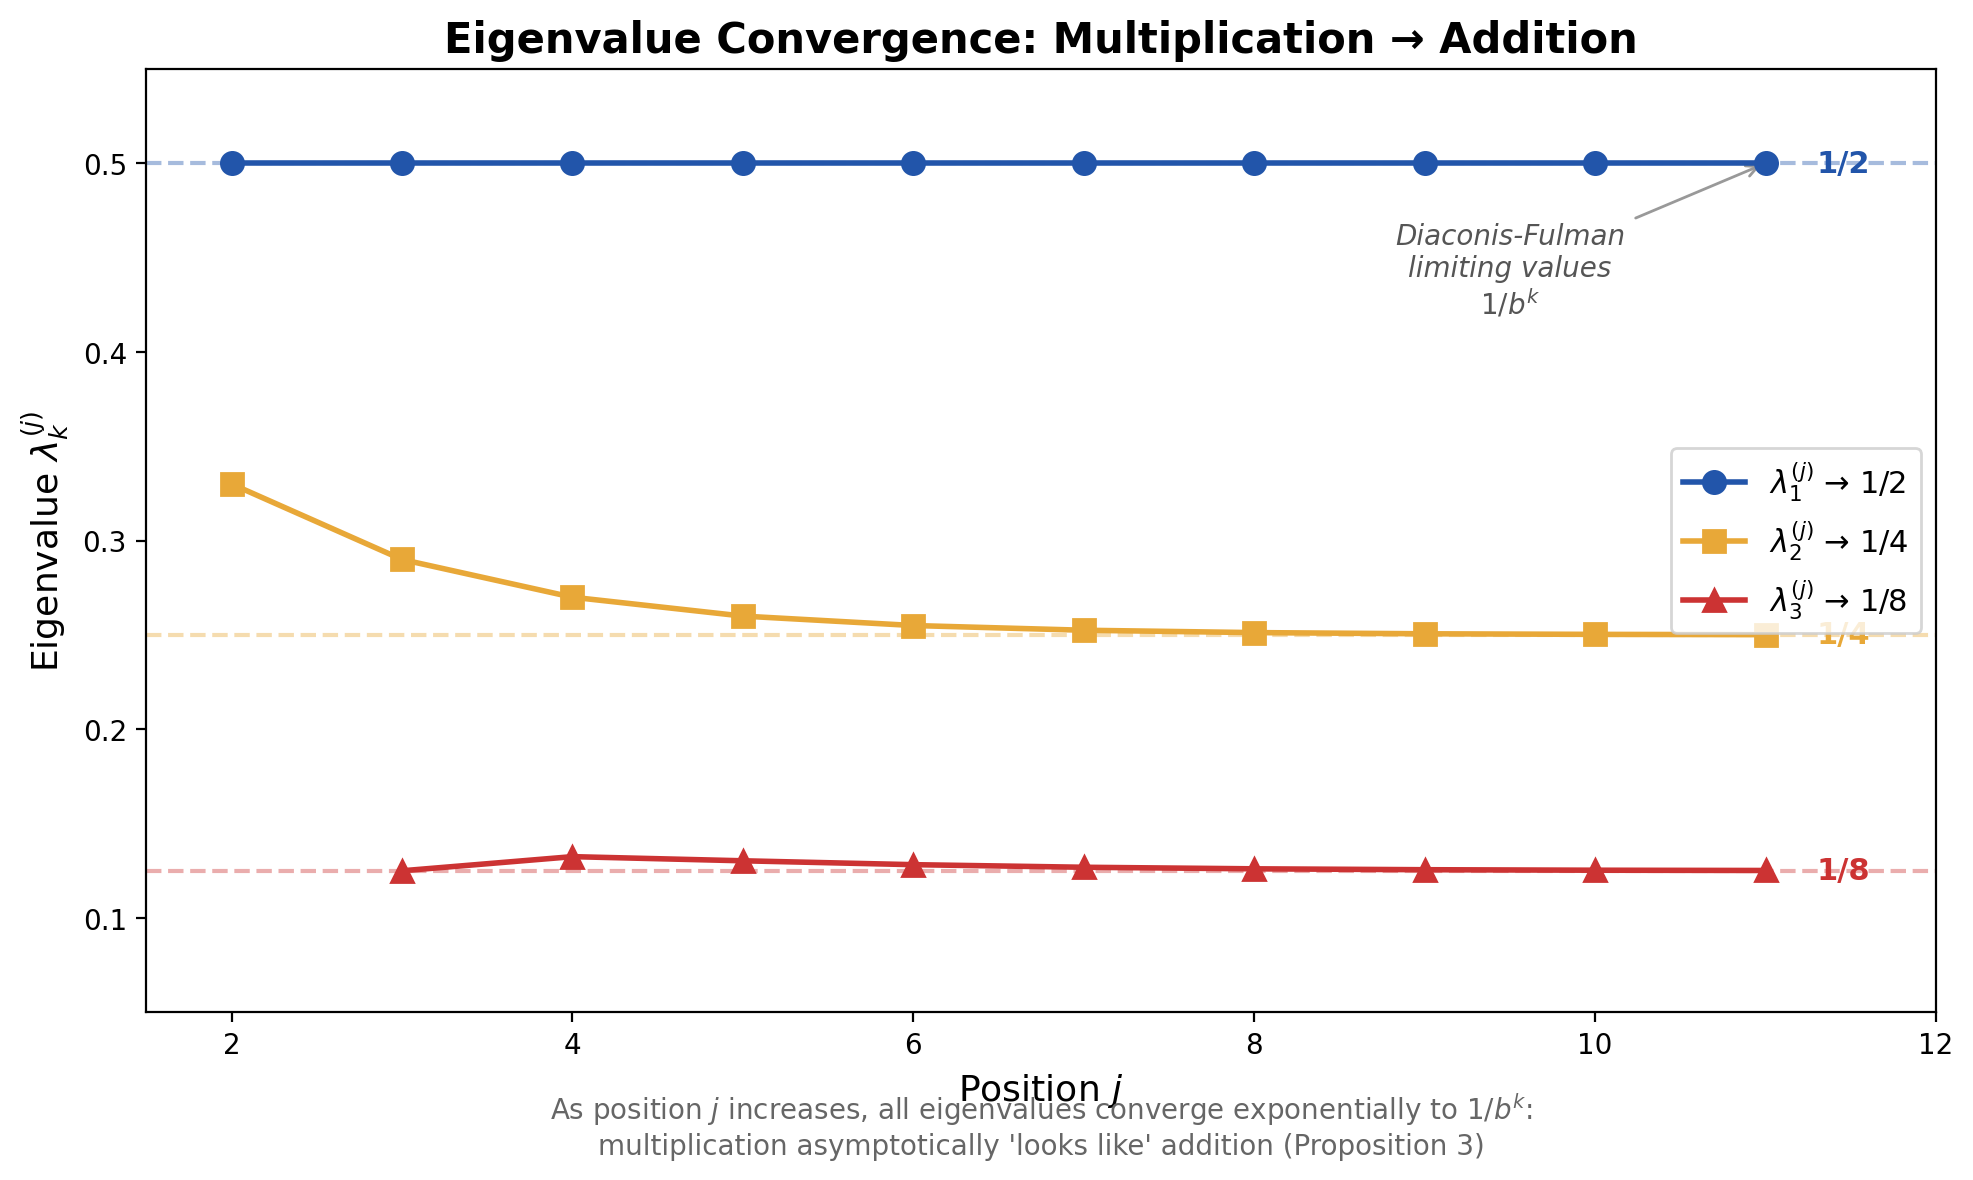
\includegraphics{../figures/fig_eigenvalue_decay.png}
\caption{Eigenvalue convergence to Diaconis-Fulman values}
\end{figure}

\subsubsection{Result 4: Spectral Radius Bound (Corollary
9)}\label{result-4-spectral-radius-bound-corollary-9}

The carry values \(c_0, c_1, \ldots, c_D\) also serve as the coefficients of a
polynomial \(Q(x)\), whose roots control an Euler-product correction series. We
prove that the spectral radius satisfies \(r_{\max} \leq 3\) for all carry
profiles with positive entries (via the Eneström-Kakeya theorem). Numerical
evidence supports the tighter conjecture \(r_{\max} \leq b\).

\begin{center}\rule{0.5\linewidth}{0.5pt}\end{center}

\newpage

\subsection{3. Connection to
Diaconis-Fulman}\label{connection-to-diaconis-fulman}

The relationship between our results and {[}1{]} can be summarized in a single
table:

\begin{longtable}[]{@{}
  >{\raggedright\arraybackslash}p{(\columnwidth - 4\tabcolsep) * \real{0.3333}}
  >{\raggedright\arraybackslash}p{(\columnwidth - 4\tabcolsep) * \real{0.3333}}
  >{\raggedright\arraybackslash}p{(\columnwidth - 4\tabcolsep) * \real{0.3333}}@{}}
\toprule\noalign{}
\begin{minipage}[b]{\linewidth}\raggedright
\end{minipage} & \begin{minipage}[b]{\linewidth}\raggedright
\textbf{Addition of \(n+1\) digits}
\end{minipage} & \begin{minipage}[b]{\linewidth}\raggedright
\textbf{Multiplication}
\end{minipage} \\
\midrule\noalign{}
\endhead
\bottomrule\noalign{}
\endlastfoot
Column sum & \(a_1^{(k)} + \cdots + a_{n+1}^{(k)}\) &
\(\sum_{i+j=k} g_i h_j\) \\
Uniform-mod-\(b\) components & \(n+1\) (all terms) & \(2\) (the ``endpoint''
terms \(g_k h_0, g_0 h_k\)) \\
Exact eigenvalues & \(1, 1/b, \ldots, 1/b^{n}\) & \(1, 1/b, 1/b^2\) (at each
position \(j \geq 2\)) \\
Higher eigenvalues & none (spectrum is complete) & \(\to 1/b^k\) exponentially
as position \(j \to \infty\) \\
State space & fixed (\(\lbrace{}0, \ldots, n\rbrace{}\) for addition of \(n+1\)
digits) & grows with position \\
Mixing time & \(O(\log n)\) & \(O(\log c_{\max})\) \\
\end{longtable}

The key insight: the \emph{mechanism} is the same --- Bernoulli smoothing of the
Fourier modes of the carry distribution --- but the \emph{count} of uniform
components differs (2 vs.~\(n+1\)), which truncates the exact spectrum.

Diaconis and Fulman {[}1, §6{]} mention that ``carries in multiplication are
more complex'' but do not develop the spectral theory. The present paper
provides this development.

\begin{center}\rule{0.5\linewidth}{0.5pt}\end{center}

\newpage

\subsection{4. Connection to Riffle
Shuffling}\label{connection-to-riffle-shuffling}

Diaconis and Fulman showed that the eigenvalues \(1/b^k\) of the addition-carry
chain are identical to those of the Gilbert-Shannon-Reeds riffle shuffle. This
is not a coincidence: both processes involve a uniform-mod-\(b\) averaging that
eliminates one degree of polynomial oscillation per step.

In our proof of the \(m\)-Bit Equidistribution Lemma, the central operator is:

\[\mathcal{A}\varphi(u) = \frac{1}{b}\sum_{j=0}^{b-1}\varphi(u+j)\]

This averages the function \(\varphi\) over a uniform shift --- structurally
analogous to the operation that governs descent statistics in the shuffle
analysis. The difference: in addition (or shuffling), this averaging is applied
\(n\) times (once per digit/card packet), giving \(n+1\) eigenvalues. In
multiplication, only 2 of the column-sum terms provide this exact averaging,
limiting the exact eigenvalues to 3. The remaining terms provide approximate
(exponentially decaying) smoothing instead of exact smoothing.

This structural parallel suggests that the spectral theory of multiplication
carries may have further connections to the algebraic combinatorics of shuffles
--- in particular, to the descent algebra of the symmetric group, where the
eigenvalues \(1/b^k\) arise as characters.

\begin{center}\rule{0.5\linewidth}{0.5pt}\end{center}

\newpage

\subsection{5. Open Directions}\label{open-directions}

Two conjectures remain open and would be natural targets for further work:

\begin{enumerate}
\def\labelenumi{\arabic{enumi}.}
\item
  \textbf{The \((b-1)/b\) Anti-Correlation Law (Conjecture 4).} Near the top of
  the multiplication (the most-significant-bit boundary), the carry increments
  \(\alpha_k\) overshoot their bulk value \((b-1)/(2b)\) and converge
  oscillatorily at rate \((b-1)/b\). This has been verified to high precision
  across millions of samples and 18 different bases, but is not proved. The
  missing step is a \emph{boundary transfer theorem} extending the covariance
  induction of {[}F{]} from the bulk to the MSB-conditioned regime.
\item
  \textbf{Tight spectral radius bound (Conjecture 10).} The proved bound
  \(r_{\max} \leq 3\) (Corollary 9) should be improvable to \(r_{\max} \leq b\).
  Numerical evidence is very strong (no counterexample in \(>10^7\) tests), but
  the Rouché-style argument has a gap at the critical radius.
\end{enumerate}

Both conjectures are accessible with current techniques and would complete the
spectral picture.

\begin{center}\rule{0.5\linewidth}{0.5pt}\end{center}

\newpage

\subsection{References}\label{references}

\begin{enumerate}
\def\labelenumi{\arabic{enumi}.}
\tightlist
\item
  P. Diaconis, J. Fulman, ``Carries, Shuffling, and Symmetric Functions,''
  \emph{Adv. Appl. Math.} 43(2), 176--196, 2009.
\item
  J. Holte, ``Carries, Combinatorics, and an Amazing Matrix,'' \emph{Amer. Math.
  Monthly} 104(2), 138--149, 1997.
\item
  {[}E{]} S. Alimonti, ``The Trace Anomaly of Binary Multiplication,'' this
  series.
  doi:\href{https://doi.org/10.5281/zenodo.18895604}{10.5281/zenodo.18895604}
  ---
  \href{https://github.com/stefanoalimonti/carry-arithmetic-E-trace-anomaly}{GitHub}
\item
  {[}F{]} S. Alimonti, ``Exact Covariance Structure of Binary Carry Chains,''
  this series.
  doi:\href{https://doi.org/10.5281/zenodo.18895607}{10.5281/zenodo.18895607}
  ---
  \href{https://github.com/stefanoalimonti/carry-arithmetic-F-covariance-structure}{GitHub}
\item
  {[}B{]} S. Alimonti, ``Carry Polynomials and the Euler Product,'' this series.
  doi:\href{https://doi.org/10.5281/zenodo.18895597}{10.5281/zenodo.18895597}
  ---
  \href{https://github.com/stefanoalimonti/carry-arithmetic-B-zeta-approximation}{GitHub}
\end{enumerate}

\begin{center}\rule{0.5\linewidth}{0.5pt}\end{center}

\emph{CC BY 4.0}

\end{document}
